\section{Design}
For this project we had to arrange several deliverables, each one with a strict deadline.
In particular:
\begin{enumerate}
\item RASD - 06/11/2015
\item DD - 04/12/2015
\item INSPECTION - 05/01/2016
\item INTEGRATION TESTING - 21/01/2016
\item PROJECT PLANNING - 02/02/2016
\end{enumerate}

To accomplish the work we folllowed the instructions of each assignment, referring 
to course material and past years projects.\\
Our team strategy was definying  all together the main guidelines of the document to be created, with one 
scribe. Then at home each of us expanded and clarified the content previously decided.\\
A special case was the inspection document, when we associated randomly the points in the checklist to each member.\\
The whole project lasted 4 months, with an individual work of 110 hours/person approximately.

\begin{center}
\begin{figure} [h]

\noindent\makebox[\textwidth]{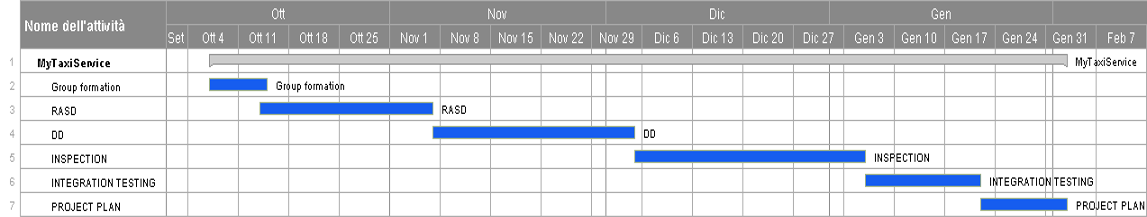
\includegraphics[scale=0.4]{chapters/SWE2-4.png}}
\caption{Gantt's diagram (design phase)}
\vspace{6mm}
\noindent\makebox[\textwidth]{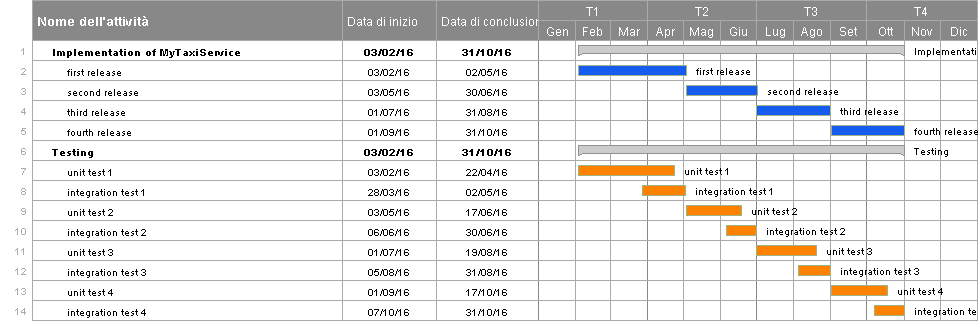
\includegraphics[scale=0.4]{chapters/Gestione Progetti(2).png}}
\caption{Gantt's diagram (implementation phase)}
%    __    __
%   >° \__/// 
%    \__ __/
%      _||
%
%  kotori-chan saw you talking with senpai
%  kotori-chan is not pleased

 \end{figure}
\end{center}

\section{Implementation}
The following section describes the partitioning of the implementation tasks, in compliance to
the project's design document and COCOMO II's data. \\
The job will be distributed to 2 developers, and the project will be split up into
smaller releases.
Every release is scheduled in the same way: an initial phase, during which development of code and unit tests
are carried out in parallel; an intermediate phase, in which integration tests begin, and a final phase, when
unit tests are completed and the code is fixed as needed. \\
More precisely, the plan includes 4 releases:
\begin{enumerate}
 \item In the first release, we aim to provide a prototype of the application, capable of executing the basic operations;
 \textit{developer 1} is tasked with writing the client-side ``major classes'', including the ones devoted to the graphic
 user interface; on top of that, (s)he will also add \textit{actions} and \textit{activities}, which allow to call a taxi,
 append it to a queue and responding to a call; \\
 \textit{developer 2} is tasked with the server-side logic, required for the correct working of the client functions,
 but this first release will feature only a single \textit{universal user}. (s)he will also work on the map-service
 integration. \\
 Each developer will also test their own components.
 \item In the second release, \textit{developer 1} is tasked with adding support for the user-management activities
 (i.e. login, logout) and the \textit{master terminal} user interface. \\
 \textit{developer 2} will work on the server-side user management. \\
 Each developer is still required to test their own components, but, given the significative job already assigned to
 \textit{developer 2}, \textit{developer 1} will work on the integration tests. \\
 This version is already deliverable to the end users, albeit with missing features.
 \item In the third release, \textit{reservations} and \textit{shared rides} will be implemented, following the
 same work distribution as before (\textit{developer 1} on the client, \textit{developer 2} on the server, each one
 write their own tests)
 \item Finally, \textit{developer 1} will implement the \textit{report} system and the \textit{ride cost calculation} system,
 while \textit{developer 2} will implement the \textit{API}.
\end{enumerate}


